\chapter{Codici}

Sia $A$ un alfabeto. Un insieme $X \subseteq A^{+}$è un codice su $A$ se ogni parola in $A^{*}$ ha al più una fattorizzazione in parole di $X$.

Formalmente, per ogni $n, m \geq 0$ e $x_{1}, \ldots, x_{n}, x_{1}^{\prime}, \ldots, x_{m}^{\prime} \in X$, la condizione
$$
x_{1} x_{2} \cdots x_{n}=x_{1}^{\prime} x_{2}^{\prime} \cdots x_{m}^{\prime}
$$
implica
$$
n=m \quad \text { e } \quad x_{i}=x_{i}^{\prime} \quad \text { per } \quad i=1, \ldots, n .
$$

\vspace{5mm}

In altre parole, un insieme $X$ è un codice se ogni parola in $X^{+}$può essere scritta in un sol modo come prodotto di parole in $X$, cioè, ha un'unica fattorizzazione in parole in $X$.

In particolare, un codice non contiene mai la parola vuota $1 .$
E chiaro che ogni sottoinsieme di un codice è un codice. In particolare, l'insieme vuoto è un codice.

\section{Fattori, prefissi, suffissi}

\begin{itemize}
    \item Una parola $w \in A^{*}$ è un fattore di una parola $x \in A^{*}$ se esistono $u, v \in A^{*}$ tali che $x=u w v$.
    
Il fattore $w$ è chiamato proprio se $w \neq x$.
    \item Una parola $w \in A^{*}$ è un prefisso di una parola $x \in A^{*}$ se esiste una parola $u \in A^{*}$ tale che $x=w u$.
    
Il prefisso $w$ è chiamato proprio se $w \neq x$.
    \item Simmetricamente una parola $w \in A^{*}$ è un suffisso di una parola $x \in A^{*}$ se esiste una parola $u \in A^{*}$ tale che $x=u w$. 
    
    Il suffisso $w$ è chiamato proprio se $w \neq x$.
\end{itemize}

\textbf{Esempio.}

Per ogni alfabeto $A$, l'insieme $X=A$ è un codice.
Più in generale, se $p \geq 1$ è un intero, allora $X=A^{p}$ è un codice chiamato il codice uniforme delle parole di lunghezza $p$ su $A$. Infatti, se elementi di $X$ soddisfano l'equazione:
$$
x_{1} x_{2} \cdots x_{n}=x_{1}^{\prime} x_{2}^{\prime} \cdots x_{m}^{\prime}
$$
allora la lunghezza costante delle parole in $X$ implica la conclusione:
$$
n=m \quad \text { e } \quad x_{i}=x_{i}^{\prime} \text { per } i=1, \ldots, n .
$$

\vspace{5mm}

\textbf{Esempio.}

Su un alfabeto che consiste di una singola lettera $a$, un sottoinsieme non vuoto $\mathrm{di} a^{*}$ è un codice se e solo se è un singoletto distinto da $1 .$
Infatti sia $X \subseteq a^{*} .$ Se $a^{h}, a^{k} \in X$, con $h \neq k$, allora la parola $w=a^{h+k}$ ha due distinte fattorizzazioni
$$
w=\left(a^{h}\right) a^{k}=a^{k}\left(a^{h}\right)
$$

\vspace{5mm}

\textbf{Esempio (1).}

$L$ 'insieme $X=\{a a, b a a, b a\}$ su $A=\{a, b\}$ è un codice.
Infatti, supponiamo il contrario. Allora esiste una parola $w$ in $X^{+}$, di lunghezza minimale, che ha due distinte fattorizzazioni,
$$
w=x_{1} x_{2} \cdots x_{n}=x_{1}^{\prime} x_{2}^{\prime} \cdots x_{m}^{\prime}
$$
$\left(n, m \geq 1, x_{i}, x_{j}^{\prime} \in X\right)$. Poiché $w$ è di lunghezza minimale, abbiamo $x_{1} \neq x_{1}^{\prime} .$

Quindi $x_{1}$ è un prefisso proprio di $x_{1}^{\prime}$ o viceversa. Assumiamo che $x_{1}$ sia un prefisso proprio di $x_{1}^{\prime}$.

\subsubsection{Esempio (2) - Inizio di una doppia fattorizzazione}

\begin{figure}[hbpt!]
    \centering
    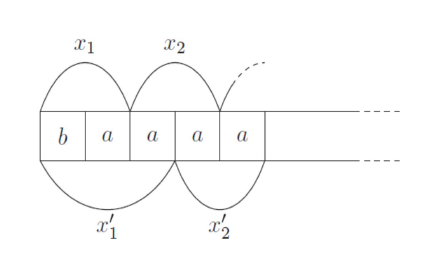
\includegraphics[width=6cm]{./Images/10.1.png}
\end{figure}
\FloatBarrier

\textbf{Esempio (3).}

Esaminando $X$, questo implica che $x_{1}=b a, x_{1}^{\prime}=$ baa.
A sua volta, questo implica che $x_{2}=a a, x_{2}^{\prime}=a a$.

Allora $x_{1}^{\prime}=x_{1} a, x_{1}^{\prime} x_{2}^{\prime}=x_{1} x_{2} a$, e se assumiamo che $x_{1}^{\prime} x_{2}^{\prime} \cdots x_{p}^{\prime}=x_{1} x_{2} \cdots x_{p} a$, segue necessariamente che $x_{p+1}=a a$ and $x_{p+1}^{\prime}=a a$.

Quindi $x_{1}^{\prime} x_{2}^{\prime} \cdots x_{m}^{\prime}=x_{1} x_{2} \cdots x_{m}$ a. Ma questo contraddice l'esistenza di due fattorizzazioni.

\vspace{5mm}

\textbf{Esempio.}

L'insieme $X=\{a, a b, b a\}$ non è un codice poiché la parola $w=a b a$ ha due distinte fattorizzazioni
$$
w=(a b) a=a(b a)
$$

\section{Piccoli codici}

Sia $X=\left\{x_{1}, x_{2}\right\} .$ Allora $X$ è un codice se e solo se $x_{1}$ e $x_{2}$ non sono potenze della stessa parola.


Nota che questa proposizione descrive interamente i codici con due elementi. Il caso di insiemi con tre parole è già molto più complicato.

\section{Richiami di algebra}
\begin{itemize}
    \item Un semigruppo è un insieme con un'operazione binaria associativa. In genere, l'operazione è denotata moltiplicativamente.
    \item Un monoide è un semigruppo che, in più, ha un elemento neutro. L'elemento neutro di un monoide $M$ è unico ed è denotato $1_{M}$ o semplicemente $1 .$
    \item Un morfismo da un monoide $M$ in un monoide $N$ è una funzione $\varphi: M \rightarrow N$ che soddisfa, per ogni $m, m^{\prime} \in M$,
$$
\varphi\left(m m^{\prime}\right)=\varphi(m) \varphi\left(m^{\prime}\right)
$$
e inoltre
$$
\varphi\left(1_{M}\right)=1_{N}
$$

    \item L'insieme di tutte le parole sull'alfabeto $A$ è denotato $A^{*}$ ed è munito di un'operazione associativa: la concatenazione di due parole.
    \item  La parola vuota, denotata 1 o $\epsilon$, è l'elemento neutro per la concatenazione.
    \item Quindi l'insieme $A^{*}$ delle parole è un monoide. II monoide $A^{*}$ è chiamato il monoide libero su $A$.
    \item Siano $A, B$ due alfabeti. Una funzione $\varphi: A \rightarrow B^{*}$ può essere estesa in modo unico a un morfismo $\varphi: A^{*} \rightarrow B^{*}$ ponendo, per ogni $w=a_{1} a_{2} \cdots a_{n}$, con $a_{i} \in A$,
$$
\varphi(w)=\varphi\left(a_{1}\right) \varphi\left(a_{2}\right) \cdots \varphi\left(a_{n}\right)
$$
    \item Ogni morfismo $\varphi: A^{*} \rightarrow B^{*}$ può essere definito in questo modo, cioè specificando la sua azione solo su $A$.
    \item Esempio. Siano $A=\{c, a, s\}$ e $B=\{a, e, r, o\}$. Poniamo
$$
\varphi(c)=\operatorname{aer}, \quad \varphi(a)=1, \quad \varphi(s)=e o .
$$
Allora $\varphi($ casa $)=$ aereo.

\end{itemize}


\subsubsection{Una diversa definizione di codice}
Se un sottoinsieme $X$ di $A^{*}$ è un codice, allora ogni funzione biettiva da un qualsiasi alfabeto $B$ su $X$ si estende a un morfismo iniettivo da $B^{*}$ in $A^{*}$. Viceversa, se esiste un morfismo iniettivo $\beta: B^{*} \rightarrow A^{*}$ tale che $X=\beta(B)$, allora $X$ è un codice.ù
\begin{itemize}
    \item  Un morfismo $\beta: B^{*} \rightarrow A^{*}$ che è iniettivo e tale che $X=\beta(B)$, è chiamato un morfismo di codifica for $X$.
    \item Per ottenere un morfismo di codifica per un codice $X \subseteq A^{*}$ basta prendere una qualsiasi funzione biettiva da un insieme $B$ su $X$ ed estenderla a un morfismo da $B^{*}$ in $A^{*}$.
\end{itemize}
Esempio. Siano $A=\{c, a, s\}$ e $B=\{a, e, r, o\}$.
\begin{itemize}
    \item Poniamo
$$
\varphi(c)=\operatorname{aer}, \quad \varphi(a)=1, \quad \varphi(s)=e o .
$$
Allora $\varphi($ casa $)=$ aereo $=\varphi($ caasa $)$. Quindi $\varphi$ non è iniettivo e $\varphi(A)=\{$ aer $, 1, e o\}$ non è un codice.
\item Poniamo
$$
\psi(c)=\operatorname{aer}, \quad \psi(a)=e, \quad \psi(s)=0 .
$$
Allora $\psi$ è iniettivo e $\psi(A)=\{$ aer $, e, o\}$ è un codice.
\end{itemize}

Per ottenere un morfismo di codifica per un codice $X \subseteq A^{*}$ basta prendere una qualsiasi funzione biettiva da un insieme $B$ su $X$ ed estenderla a un morfismo da $B^{*}$ in $A^{*}$.

In questo contesto, l'alfabeto $B$ è chiamato l'alfabeto sorgente mentre l'alfabeto $A$ è l'alfabeto del canale.

La proposizione precedente è l'origine della terminologia poiché le parole in $X$ codificano le lettere dell'insieme $B$. La codifica consiste nell'associare a una parola $b_{1} b_{2} \cdots b_{n}$ $\left(b_{i} \in B\right)$, che è il messaggio sorgente, un messaggio codificato $\beta\left(b_{1}\right) \cdots \beta\left(b_{n}\right)$ sull'alfabeto del canale, usando il morfismo di codifica $\beta$.

Il fatto che $\beta$ sia iniettiva assicura che il testo codificato sia univocamente decifrabile, per ottenere nuovamente il testo originale.

\subsubsection{Insiemi prefissi, suffissi, bifissi}

Un'importante classe di codici è la classe dei codici prefissi.
Un sottoinsieme $X$ di $A^{*}$ è prefisso se nessun elemento di $X$ è un prefisso proprio di un altro elemento in $X$.

Dalla definizione segue immediatamente che se un insieme prefisso $X$ contiene la parola vuota 1 allora $X=\{1\}$.

\vspace{5mm}

Gli insiemi suffissi sono definiti simmetricamente.
Un sottoinsieme $X$ di $A^{*}$ è suffisso se nessuna parola in $X$ è un suffisso proprio di un'altra parola in $X$.
Un insieme è bifisso se è prefisso e suffisso.

Chiaramente, un insieme di parole $X$ è suffisso se e solo se il suo reverse $\widetilde{X}=\{\tilde{w} \mid w \in X\}$ è prefisso.
Se $w=a_{1} a_{2} \cdots a_{n}$, con $a_{i} \in A$
$$
\tilde{w}=a_{n} \cdots a_{2} a_{1}
$$

\subsubsection{Codici prefissi, suffissi, bifissi}
Ogni insieme prefisso (suffisso, bifisso) di parole $X \neq\{1\}$ è un codice.


\vspace{5mm}

Dimostrazione.

Poiché $X \neq\{1\}, X$ non contiene la parola vuota.
Se $X$ non fosse un codice, ci sarebbe una parola $w$ di lunghezza minimale con due fattorizzazioni
$$
w=x_{1} x_{2} \cdots x_{n}=x_{1}^{\prime} x_{2}^{\prime} \cdots x_{m}^{\prime} \quad\left(x_{i}, x_{j}^{\prime} \in X\right)
$$
Le stringhe $x_{1}, x_{1}^{\prime}$ sono diverse dalla parola vuota, e poiché $w$ ha lunghezza minimale, $x_{1} \neq x_{1}^{\prime}$.

Ma allora $x_{1}$ è prefisso proprio di $x_{1}^{\prime}$ oppure $x_{1}^{\prime}$ è prefisso proprio di $x_{1}$, in contraddizione con il fatto che $X$ è prefisso. Quindi $X$ è un codice.

Nella prova abbiamo considerato un insieme prefisso $X \neq\{1\}$.
L'argomento è lo stesso se $X \neq\{1\}$ è un insieme suffisso ma applicato a $ x_{n}=x_{m}^{\prime}$.

\vspace{5mm}

Un codice prefisso (codice suffisso, codice bifisso) è un insieme prefisso (insieme suffisso, insieme bifisso) che è un codice, cioè che è distinto da $\{1\}$.

Quindi un codice prefisso è un insieme $X \subseteq A^{+}$tale che nessuna parola di $X$ è un prefisso di un'altra parola di $X$.

Simmetricamente, un codice suffisso è un insieme $X \subseteq A^{+}$tale che nessuna parola di $X$ è un suffisso di un'altra parola di $X$.

Un codice bifisso è un codice prefisso e suffisso.

\subsubsection{Esempio}

I codici uniformi sono bifissi.
L'insieme $X=\{a, b a\}$ è un codice prefisso e $Y=\{a, a b\}$ è un codice suffisso.

\subsubsection{Esempio}

Gli insiemi $X=L\left(a^{*} b\right)$ e $Y=\left\{a^{n} b^{n} \mid n \geq 1\right\}$ su $A=\{a, b\}$ sono prefissi, quindi codici prefissi.

L'insieme $Y$ è suffisso, quindi è un codice bifisso.
Invece $X$ non è suffisso, per esempio $b$ è un suffisso proprio di $a b$.
Questo esempio mostra l'esistenza di codici infiniti su un alfabeto finito.

\subsubsection{Esempio}

II codice Morse associa a ogni carattere alfanumerico una sequenza di punti e linee.

Per esempio, la codifica di $A$ è ". -" la codifica di J è ". - - -".

Se conveniamo che ciascuna parola di codice termina con un simbolo addizionale (in genere uno spazio, chiamato una "pausa"), il codice Morse diventa un codice prefisso.

\subsubsection{Ordine radix}

Sia $\Sigma=\left\{a_{0}, \ldots, a_{k}\right\}$ un alfabeto e sia $a_{0}<a_{1}<\ldots<a_{k}$ un ordinamento degli elementi di $\Sigma$. Siano $x, y \in \Sigma^{*}$.

Diremo che $x \leq y$ rispetto all'\textbf{ordine radix} se $x$ e $y$ verificano una delle condizioni seguenti:
\begin{enumerate}
\item  $|x|<|y|$.
\item  $|x|=|y|$ e $x=z a x^{\prime}, y=z b y^{\prime}, \operatorname{con} z, x^{\prime}, y^{\prime} \in \Sigma^{*}, a, b \in \Sigma$ e $a \leq b$.
\end{enumerate}

In "Introduzione alla teoria della computazione", l'ordine radix è chiamato \textbf{ordine per lunghezza}.
La lista dei numeri in base $k$ in ordine crescente è una lista di stringhe su $\Sigma=\{0, \ldots, k-1\}$ in ordine radix.
\begin{itemize}
    \item Esempio. Supponiamo $a<b<\ldots<z$.
    
barca $<$ aurora, castagna $<$ castello.
    \item La lista delle stringhe su $\Sigma=\{0,1\}$, con $0<1$, in ordine radix:
$$
\epsilon, 0,1,00,01,10,11,000,001,010,011,100, \ldots
$$
    \item La lista delle stringhe su $\Sigma=\{a, b, c\}$, con $a<b<c$, in ordine radix:
$$
\epsilon, a, b, c, a a, a b, a c, b a, b b, b c, c a, c b, c c, \ldots
$$
\end{itemize}

\subsubsection{Codici prefissi}

Esiste un'utile rappresentazione grafica dei codici prefissi.
Questa rappresentazione consiste nell'associare un albero a un
codice prefisso tale che le parole nel codice sono rappresentate da
foglie dell'albero.

\subsubsection{Grafo di Cayley di $A^*$}

Innanzitutto, associamo un albero infinito all'insieme $A^{*}$ delle parole su un alfabeto $A$ nel seguente modo.

L'alfabeto è totalmente ordinato e le parole di uguale lunghezza sono ordinate mediante l'ordine radix.
ù
Ogni nodo dell'albero rappresenta una parola in $A^{*}$. Ogni parola è alla sinistra delle parole di lunghezza maggiore e le parole di uguale lunghezza sono disposte verticalmente secondo l'ordine radix.

C'è un arco da $u$ a $v$ se e solo se $v=u a$ per qualche lettera $a \in A$.
L'albero ottenuto in questo modo è la rappresentazione letterale di $A^{*}$ ed è anche chiamato il grafo di Cayley di $A^{*}$.

\subsubsection{Grafo di Cayley di $\{a, b\}^{*}$ e di $\{a, b, c\}^{*}$}

\begin{figure}[hbpt!]
    \centering
    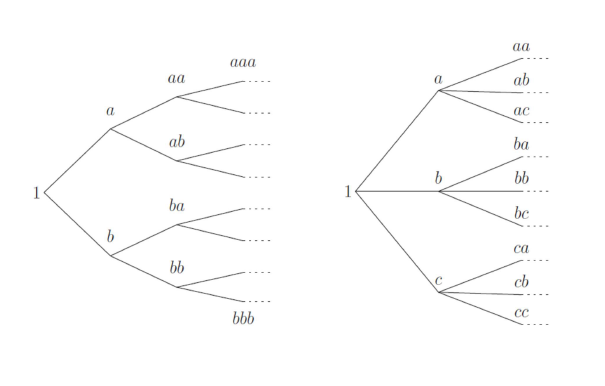
\includegraphics[width=8cm]{./Images/10.2.png}
\end{figure}
\FloatBarrier

\subsubsection{Rappresentazione mediante alberi}

A un sottoinsieme $X$ di $A^{*}$ associamo un sottoalbero del grafo di Cayley di $A^{*}$ nel seguente modo.
Prendiamo solo i nodi che corrispondono alle parole in $X$ e tutti i nodi sui cammini dalla radice a questi nodi.
L'albero ottenuto in questo modo è la \textit{rappresentazione letterale} $\mathrm{di} X$.

\subsubsection{Rappresentazione letterale di $X=\{a, b a, b a a\}$ (con etichette)}

\begin{figure}[hbpt!]
    \centering
    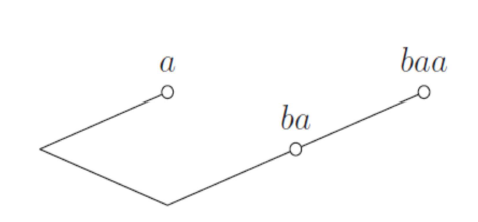
\includegraphics[width=7cm]{./Images/10.3.png}
\end{figure}
\FloatBarrier

\subsubsection{Rappresentazione letterale di $X=\{a, b a, b a a\}$ (senza etichette)}

\begin{figure}[hbpt!]
    \centering
    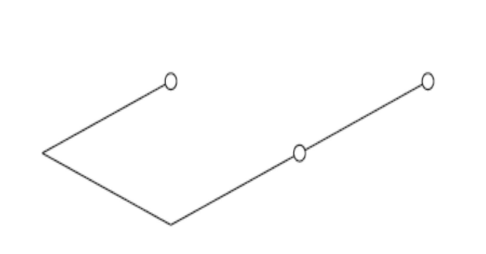
\includegraphics[width=7cm]{./Images/10.4.png}
\end{figure}
\FloatBarrier

Una rappresentazione grafica alternativa consiste nel disegnare l'albero dall'alto al basso invece che da sinistra a destra.

In questo caso, le parole di ugual lunghezza sono disposte orizzontalmente da sinistra a destra in base all'ordine radix.

\subsubsection{Rappresentazione letterale di $X=L\left(a^{*} b\right)$ (sinistra-destra e top-down)}

\begin{figure}[hbpt!]
    \centering
    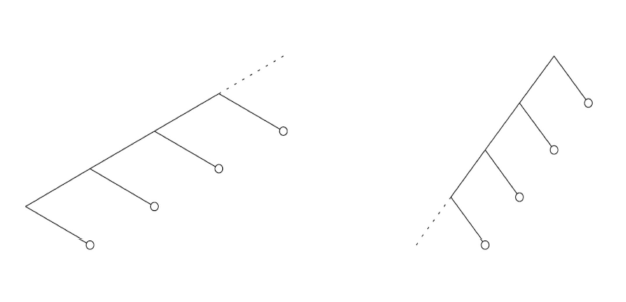
\includegraphics[width=9cm]{./Images/10.5.png}
\end{figure}
\FloatBarrier

\subsubsection{Rappresentazione letterale dei codici prefissi}

Si vede facilmente che un codice X è prefisso se e solo se nella
rappresentazione letterale di X, tutti i nodi corrispondenti alle
parole in X sono foglie dell'albero.

\vspace{5mm}

Il vantaggio della rappresentazione letterale rispetto alla semplice
enumerazione è nella facile leggibilità delle proprietà del codice.

Essa fornisce una rappresentazione compatta di codici con molti
elementi.

(a) rappresenta $X=\{a, b a a, b a b, b b\}$,

(b) rappresenta $X=\left\{b^{2}\right\}^{*}\left\{a^{2} b, b a\right\}$.

\begin{figure}[hbpt!]
    \centering
    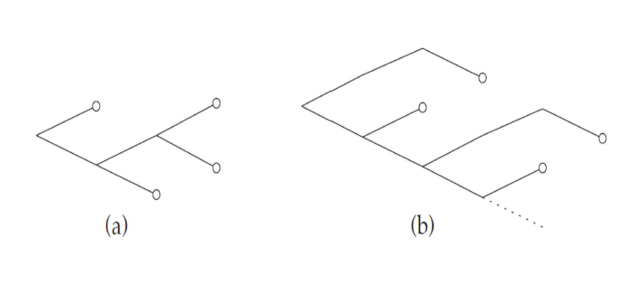
\includegraphics[width=7cm]{./Images/10.6.png}
\end{figure}
\FloatBarrier

\subsubsection{Un test per i codici}

Non è sempre semplice verificare che un dato insieme di parole è un codice.

Esiste un test che non è basato su una qualche nuova proprietà dei codici ma consiste semplicemente in una sistematica organizzazione delle computazioni richieste per verificare che un insieme di parole soddisfa la definizione di codice.

Nel caso in cui $X$ sia finito, o più generalmente se $X$ è regolare (riconoscibile), la computazione è finita. In altre parole, è decidibile se un insieme finito o regolare è un codice.

\vspace{5mm}

Illustriamo la descrizione dell'algoritmo su un esempio.
Esempio.

Sia $A=\{a, b\}$ e $X=\{b, a b b, a b b b a, b b b a, b a a b b\} .$
Questo insieme non è un codice. Per esempio $(a b b)(b a b b)=(a b b b a)(a b b)$.

Consideriamo la parola
$$
w=a b b b a b b b a a b b
$$
che ha le due fattorizzazioni
$$
w=(a b b b a)(b b b a)(a b b)=(a b b)(b)(a b b)(b a b b) .
$$

\subsubsection{Un test per i codici - Esempio}

Le due fattorizzazioni della parola $w=a b b b a b b b a b b$.

\begin{figure}[hbpt!]
    \centering
    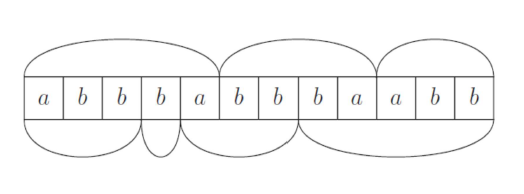
\includegraphics[width=7cm]{./Images/10.7.png}
\end{figure}
\FloatBarrier

Queste due fattorizzazioni definiscono una sequenza di prefissi di $w=a b b b a b b b a b b$, ognuna corrispondente a un tentativo di trovare una doppia fattorizzazione.
$X=\{b, a b b, a b b b a, b b b a, b a a b b\}$
$$
\begin{array}{rc}
(a b b b a) & =(a b b) b a \\
(a b b b a) & =(a b b)(b) a \\
(a b b b a) b b & =(a b b)(b)(a b b) \\
(a b b b a)(b b b a) & =(a b b)(b)(a b b) b a \\
(a b b b a)(b b b a) a b b & =(a b b)(b)(a b b)(b a a b b) \\
(a b b b a)(b b b a)(a b b) & =(a b b)(b)(a b b)(b a a b b)
\end{array}
$$
Ognuno di questi tentativi, tranne l'ultimo, fallisce a causa del suffisso sottolineato, che resta dopo la fattorizzazione.

\subsubsection{Richiami}

Per $x, y \in A^{*}$, definiamo
$$
x^{-1} y=\left\{z \in A^{*} \mid x z=y\right\} \quad \text { e } \quad x y^{-1}=\left\{z \in A^{*} \mid x=z y\right\} .
$$
Per sottoinsiemi $X, Y$ di $A^{*}$, questa notazione è estesa a
$$
X^{-1} Y=\bigcup_{x \in X} \bigcup_{y \in Y} x^{-1} y \quad e \quad X Y^{-1}=\bigcup_{x \in X} \bigcup_{y \in Y} x y^{-1}
$$
L'insieme $X^{-1} Y$ è chiamato un quoziente (o residuo) sinistro di $Y$.

La notazione $X^{-1} Y$ non deve essere confusa con il prodotto dell'inverso di un elemento con un altro in un qualche gruppo.

\subsubsection{Un test per i codici}

Formalmente, le computazioni sono organizzate come segue. Sia $X$ un sottoinsieme di $A^{+}$e sia
$$
\begin{aligned}
U_{1} &=X^{-1} X \backslash\{1\} \\
U_{n+1} &=X^{-1} U_{n} \cup U_{n}^{-1} X \quad(n \geq 1)
\end{aligned}
$$
Sussiste il teorema seguente

\vspace{5mm}

\textbf{Teorema}

L'insieme $X \subseteq A^{+}$è un codice se e solo se nessuno degli insiemi $U_{n}$ definiti sopra contiene la parola vuota.

\vspace{5mm}

Se $X \subseteq A^{+}$è prefisso (quindi è un codice), allora $U_{1}=X^{-1} X \backslash\{1\}=\emptyset$. Quindi l'algoritmo termina immediatamente per tali codici.

\textbf{Esempio.} 
Sia $A=\{a, b\}$ e $X=\{b, a b b, a b b b a, b b b a, b a a b b\} .$ La parola ba è in $U_{1}$ (utilizzando abb e abbba), poi abb $\in U_{2}$ (utilizzando ba e baabb) e poiché $1 \in U_{3}$, l'insieme $X$ non è un codice, in accordo con il teorema.

\vspace{5mm}

Per $X=\{b, a b b, a b b b a, b b b a, b a a b b\}$, otteniamo
$$
\begin{aligned}
U_{1} &=\{b a, b b a, a a b b\}, \\
X^{-1} U_{1} &=\{a, b a\}, \\
U_{1}^{-1} X &=\{a b b\}, \\
U_{2} &=\{a, b a, a b b\}, \\
X^{-1} U_{2} &=\{a, 1\}, \\
U_{2}^{-1} X &=\{b b, b b b a, a b b, 1, b a\}, \\
U_{3} &=\{a, 1, b b, b b b a, a b b, b a\} .
\end{aligned}
$$
Quindi $1 \in U_{3}$ e $X$ non è un codice.

\vspace{5mm}

\textbf{Esempio.}

Sia $X=\{a, a b, b a\}$ e $A=\{a, b\}$. Abbiamo
$$
U_{1}=\{b\}, \quad U_{2}=\{a\}, \quad U_{3}=\{1, b\} .
$$
L'insieme $U_{3}$ contiene la parola vuota. Quindi $X$ non è un codice.

\vspace{5mm}


\textbf{Esempio.}

Sia $X=\{a a, b a, b b, b a a, b b a\}$ e $A=\{a, b\} .$ Otteniamo $U_{1}=\{a\}, U_{2}=U_{1}$. Quindi $U_{n}=\{a\}$ per ogni $n \geq 1$ e X è un codice.

\vspace{5mm}

Il precedente teorema e la proposizione seguente mostrano che la proprietà di essere un codice è decidibile per un insieme regolare.


\textbf{Proposizione}
Se $X \subseteq A^{+}$è un insieme regolare, allora l'insieme di tutti gli $U_{n}$ $(n \geq 1)$ è finito.

Questo enunciato è ovvio se l'insieme $X$ è finito, poiché è facile dimostrare, utilizzando il principio di induzione, che ogni $U_{n}$ è composto di suffissi di parole in $X$.

\vspace{5mm}

\textbf{Esempio.}

Sia $A=\{a, b\}$ e $X=L\left(b a^{*}\right)$. Quindi $X$ è un codice suffisso regolare.
Risulta $U_{1}=\left\{a^{n} \mid n>0\right\}$ e $U_{2}=\emptyset$. Quindi la sequenza $\left(U_{n}\right)$ ha due elementi distinti.

\subsubsection{Codici massimali}

Un codice $X$ è massimale su $A$ se $X$ non è propriamente contenuto in alcun altro codice su A, ovvero, se
$$
X \subseteq X^{\prime}, \quad X^{\prime} \text { codice } \Rightarrow X=X^{\prime}
$$

La massimalità di un codice dipende dall'alfabeto su cui è data. Infatti, se $X \subseteq A^{*}$ e $A$ è incluso strettamente in $B$, allora $X \subseteq B^{*}$ e $X$ è certamente non massimale su $B$, anche se è un codice massimale su $A$.

La definizione di massimalità non suggerisce un algoritmo che permetta di verificare se un codice sia o meno massimale.
Ma la massimalità è decidibile per i codici regolari.

\vspace{5mm}

\textbf{Esempio.}

I codici uniformi $A^{n}$ sono massimali su $A$.
Supponiamo il contrario. Quindi esiste una parola $u \in A^{+} \backslash A^{n}$ tale che $Y=A^{n} \cup\{u\}$ è un codice.

La parola $w=u^{n}$ appartiene a $Y^{*}$ ed è anche in $\left(A^{n}\right)^{*}$ perché la sua lunghezza è un multiplo di $n$.
Quindi
$$
w=u^{n}=x_{1} x_{2} \cdots x_{|u|}
$$
$\operatorname{con} x_{1}, \ldots, x_{|u|} \in A^{n}$
Ma $u \notin A^{n}$. Quindi le due fattorizzazioni sono distinte, $Y$ non è un codice e $A^{n}$ è massimale.

\vspace{5mm}

\textbf{Proposizione}

Ogni codice $X$ su $A$ è contenuto in un codice massimale su $A$.
La prova non è costruttiva. Applica il lemma di Zorn all'insieme $\mathcal{F}$ dei codici su $A$ contenenti $X$, ordinati rispetto all'inclusione, che assicura l'esistenza di un elemento massimale in $\mathcal{F}$, se alcune condizioni sono verificate.

\vspace{5mm}

La proposizione precedente non è più vera se ci restringiamo ai codici finiti (ma è vera per i codici regolari).

Esistono codici finiti che non sono contenuti in alcun codice massimale finito.
Sarà fornito un esempio di un tale codice.

\subsubsection{Codici completi}

Un sottoinsieme $X$ di $A^{*}$ è completo se, per ogni $w \in A^{*}$,
$$
A^{*} w A^{*} \cap X^{*} \neq \emptyset \text {. }
$$

\vspace{5mm}

\textbf{Teorema}

Ogni codice massimale è completo.

\vspace{5mm}

\textbf{Teorema}

Ogni codice completo e regolare è massimale.

\subsubsection{Codici completi - conseguenze}

Esistono codici finiti che non sono contenuti in alcun codice massimale finito.

\vspace{5mm}

\textbf{Proposizione}

L'insieme $X=\left\{a^{5}, b a^{2}, a b, b\right\}$ è un codice su $A=\{a, b\} .$ Ogni codice massimale che contiene $X$ è infinito.

\vspace{5mm}

\textbf{Proposizione}

Sia $X \subseteq A^{*}$ un codice massimale finito. Per ogni sottoinsieme non vuoto $B$ di $A$, il codice $X \cap B^{*}$ è un codice massimale su $B$.
In particolare, per ogni lettera $a \in A$, esiste un intero $n$ tale che $a^{n} \in X$.

\subsubsection{Composizione di codici}

Esiste un'operazione binaria parziale sui codici chiamata composizione. Questa operazione associa a due codici $Y$ e $Z$ che soddisfano una condizione di compatibilità un terzo codice denotato con $Y \circ Z$.
C'è un doppio interesse in questa operazione.

\vspace{5mm}

In primo luogo fornisce un utile metodo per costruire codici più complessi da codici semplici. Per esempio, la composizione di un codice prefisso e un codice suffisso può produrre un codice che non è né prefisso né suffisso.

Poi, e questo costituisce l'interesse principale per la composizione, la nozione inversa di decomposizione permette di studiare la struttura dei codici. Se un codice $X$ si decompone in due codici $Y$ e $Z$, allora questi codici sono generalmente più semplici.

\subsubsection{Composizione di codici - un esempio}

Sia $X=\{$ bbaba, a abba, a abbabb $\}$ e $Z=\{a, b a, b b\} .$
Ogni elemento di $X$ è prodotto di elementi di $Z . X$ si decompone su $Z$.

Associamo a ogni elemento di $Z$ una lettera di un altro alfabeto, ad esempio $B=\{x, y, w\}$ e poniamo $\beta(x)=\mid a, \beta(y)=$ ba e $\beta(w)=(b b) .$
Sia $Y=\{w x y, x x w x, x x w x x\} .$ Allora $X=\beta(Y)$ è la composizione di $Y$ e $Z . X$ è ottenuto da $Y$ sostituendo ogni lettera in $B$ con la corrispondente parola in $Z$.

\subsubsection{Composizione di codici}

Sia $Z$ un codice sull'alfabeto $A, \operatorname{sia} \beta: B \rightarrow Z$ una biezione da un alfabeto $B$ su $Z$ e sia $Y$ un codice sull'alfabeto $B$. Allora $X=\beta(Y)$ è un codice su $A$ denotato
$$
X=Y \circ Z
$$

Diremo che $X$ è la composizione di $Y$ e $Z$.

Per esempio, sia $X=\{a a, a a b, a b, a b b, b b\}$. Sia $Z$ il codice prefisso $Z=\{a a, a b, b\} .$ Sia $B=\{u, v, w\}$ e sia $\beta: B \rightarrow Z$ tale che $\beta(u)=a a, \beta(v)=a b, \beta(w)=b$. Allora $X=Y \circ Z$ dove $Y$ è il codice suffisso $Y=\{u, v, u w, v w, w w\}$.

\vspace{5mm}

Consideriamo ora il secondo aspetto dell'operazione di composizione, la decomposizione di un codice in codici più semplici.
Abbiamo bisogno di una nozione. Sia $Z \subseteq A^{*}$ un codice e sia $X \subseteq A^{*} .$ Poniamo
$$
\operatorname{alph}_{Z}(X)=\left\{z \in Z \mid \exists u, v \in Z^{*}: u z v \in X\right\}
$$
In altre parole, $\operatorname{alph}_{Z}(X)$ è l'insieme delle parole in $Z$ che compaiono almeno una volta in una fattorizzazione di una parola in $X$ come prodotto di parole in $Z$.

\vspace{5mm}

\textbf{Proposizione}

Siano $X, Z \subseteq A^{*}$ codici. Esiste un codice $Y$ tale che $X=Y \circ Z$ se e solo se
$$
X \subseteq Z^{*} \quad e \quad \operatorname{alph}_{Z}(X)=Z
$$
La seconda condizione nella precedente equazione significa che tutte le parole in $Z$ compaiono in almeno una fattorizzazione di una parola in $X$ come prodotto di parole in $Z$.

\subsubsection{Codici e sottomonoidi}

$A$ sottomonoide di $A^{*}$ è generato da un codice se e solo se è libero, cioè è isomorfo a un monoide libero $B^{*}$ su un alfabeto $B$.

Sia $M$ un monoide. Un sottomonoide $N$ di $M$ è stabile (in $M$ ) se per ogni $u, v, w \in M$,
$$
u, v, u w, w v \in N \Rightarrow w \in N
$$
È chiamato unitario a destra se per ogni $u, w \in M$,
$$
u, u w \in N \Rightarrow w \in N
$$

\subsubsection{Rappresentazione della stabilità}

\begin{figure}[hbpt!]
    \centering
    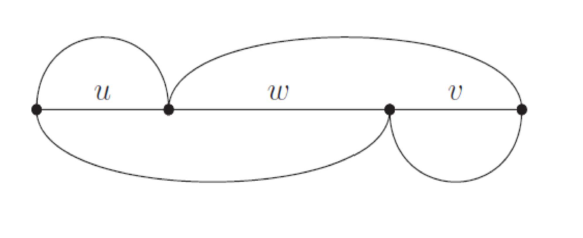
\includegraphics[width=8cm]{./Images/10.8.png}
\end{figure}
\FloatBarrier

\textbf{Proposizione}

Un sottomonoide $N$ di $A^{*}$ è stabile (risp. unitario a destra) se e solo se è generato da un codice (risp. un codice prefisso).

\subsubsection{Distribuzione di Bernoulli}

Una distribuzione di Bernoulli è un morfismo da $A^{*}$ in $[0,1]$ tale che $\sum_{a \in A} \pi(a)=1$.

Una distribuzione di Bernoulli è positiva se e solo se $\pi(a)>0$ for tutte le lettere a.
Inoltre per ogni sottoinsieme non vuoto $X$ di $A^{*}$ poniamo
$$
\pi(X)=\sum_{x \in X} \pi(x)
$$

\subsubsection{Teorema (Disuguaglianza di Kraft-McMillan generalizzata) }

Se $X$ è un codice su $A$, allora $\pi(X) \leq 1$ per ogni distribuzione di Bernoulli $\pi$ su $A^{*}$.


Esempio.
Sia $A=\{a, b\}$ e $X=\{b, a b, b a\} .$ Sia $\pi$ tale che $\pi(a)=1 / 3$, $\pi(b)=2 / 3$. Allora
$$
\pi(X)=\frac{2}{3}+\frac{2}{9}+\frac{2}{9}=\frac{10}{9}
$$
Quindi $X$ non è un codice. Nota che con $\rho(a)=\rho(b)=1 / 2$ otteniamo $\rho(X)=1$. Quindi non è possibile concludere che $X$ non è un codice usando la distribuzione $\rho$.

\vspace{5mm}

\textbf{Esempio.}
Sia $A=\{a, b\}$ e $X=\{a b, a b a, a a b\}$. L'insieme $X$ non è un codice poiché
$$
(a b a)(a b)=(a b)(a a b)
$$
Si potrebbe dimostrare che per ogni distribuzione di Bernoulli $\pi$ risulta $\pi(X)<1$.

\vspace{5mm}

\textbf{Proposizione}

Sia $X$ un codice su A. Se esiste una distribuzione positiva di Bernoulli $\pi$ su $A^{*}$ tale che $\pi(X)=1$, allora il codice $X$ è massimale.

\subsubsection{Distribuzione di Bernoulli uniforme}

La distribuzione di Bernoulli uniforme è definita da $\pi(a)=1 / \operatorname{Card}(A)$ per ogni $a \in A$.
Se l'alfabeto $A$ è finito e la distribuzione $\pi$ è uniforme otteniamo il seguente corollario

\subsubsection{Corollario (Disuguaglianza di Kraft-McMillan)}

Sia $X$ un codice su un alfabeto con $k$ lettere. Allora
$$
\sum_{x \in X} k^{-|x|} \leq 1
$$

\subsubsection{Disuguaglianza di Kraft}

Sia $S$ un insieme di parole sull'alfabeto $A$. La sequenza $s_{n}=\operatorname{Card}\left(S \cap A^{n}\right)$ è la distribuzione delle lunghezze (o funzione di struttura) dell'insieme $S$.

\vspace{5mm}


\textbf{Teorema (Kraft, 1956)}


Una sequenza $u_{n}$ di interi è la distribuzione delle lunghezze di un codice su $k$ lettere se e solo se $\sum_{n} u_{n} k^{-n} \leq 1$.
Non è difficile vedere che se la disuguaglianza di Kraft è soddisfatta esiste un codice prefisso $X$ su un alfabeto a $k$ lettere tale che $u_{n}=\operatorname{Card}\left(X \cap A^{n}\right)$.


\subsubsection{Codici circolari}

Un codice circolare è un insieme $X \subseteq A^{+}$tale che ogni parola scritta su un cerchio ha al più una fattorizzazione in parole di $X$.

Formalmente, per ogni $x_{1}, \ldots, x_{n}$ e $y_{1}, \ldots, y_{m}$ in $X$ e $p \in A^{*}$, $s \in A^{+}$, si ha
$$
s x_{2} \cdots x_{n} p=y_{1} \cdots y_{m}, x_{1}=p s
$$
solo se $n=m, p=1$, e $x_{i}=y_{i}$ per $i=1, \ldots, n$.
Un sottomonoide $M$ di $A^{*}$ è \textbf{molto puro} se per ogni $u, v \in A^{*}$,
$$
u v, v u \in M \Rightarrow u, v \in M
$$

\subsubsection{Due fattorizzazioni circolari}

\begin{figure}[hbpt!]
    \centering
    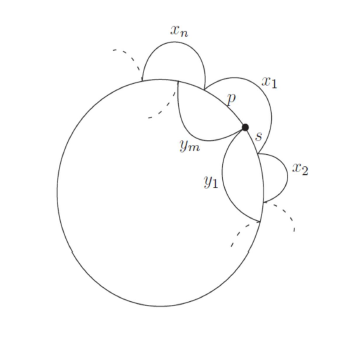
\includegraphics[width=6cm]{./Images/10.9.png}
\end{figure}
\FloatBarrier

\textbf{Proposizione}

Un sottomonoide di $A^{*}$ è molto puro se e solo se il suo insieme minimale di generatori è un codice circolare.

\subsubsection{Composizione di codici circolari}

La composizione di due codici circolari è un codice circolare.
Segue dal fatto che se $N \subseteq M \subseteq A^{*}$, dove $N$ è un sottomonoide molto puro di $M$ e $M$ è un sottomonoide molto puro di $A^{*}$, allora $N$ è un sottomonoide molto puro di $A^{*}$.




\let\cleardoublepage\clearpage

